 
\textbf{Power Ambience Dynamics : }
We bifurcate the types of sensors into two measurement categories namely ambience and electric power.


Next we investigate into a special configuration that approximates a bidirectional mapping between two sub-groups: power$(g_p)$, and ambience $(g_a)$.
We hypothesize that power dissipation and ambient conditions share a causality relation and give some supporting examples.
When Air Conditioning unit is turned on, then indoor temperature will tend to meet the set point target.
In an office space, ideally there should not be overhead tube-lights or bulbs or desktop monitors turned on , after working hours.

 

\begin{algorithm}
\caption{Optimize Virtual Sensor Field }\label{alg:chromAccuracy}
\begin{algorithmic}
\Require Chromosome Pool $\{B^c\}$, Memory Table $M$, Groups $G$, Objectives \textbf{O}
% \Ensure $W = |diag (M_k^g)| \forall k \in \tau, g \in G$
\State $L \gets 0$
\State $i \gets 0$
\State 
\For{$g \in G$} \Comment{Iterate over tasks}
\While{$i  <N$} \Comment{Iterate on Chromosome }
\State S = ${j | j \in A^c[i:i+W], V( A^c[j])=1}$
\State A = ${j | j \in A^c[i:i+W], V( A^c[j])=0}$
\For{$s \in S$}
\For{$a \in A$}
\State $g \gets G[\lceil{\frac{i}{W}} \rceil]$ \Comment{Select Group}
\State L $ \gets L + M_k^g[s,a]$
\EndFor
\EndFor
\State $i \gets i + W$
\EndWhile
\EndFor
\State return L
\end{algorithmic}
\end{algorithm}


\begin{table}[]
\begin{tabular}{|l|l|l|l|l|l|}
\hline
Nodes     & Floor      & \multicolumn{2}{l|}{$\mathcal{F}_{p2a}$ } & \multicolumn{2}{l|}{$\mathcal{F}_{a2p}$  } \\ \hline
\multicolumn{2}{|l|}{} & MSE           & MAE          & MSE           & MAE          \\ \hline
13        & 4,5,6,7    &               &              &               &              \\ \hline
10        & 4,5,6      &               &              &               &              \\ \hline
7         & 6,7        &               &              &               &              \\ \hline
4         & 6          &               &              &               &              \\ \hline
\end{tabular}
\caption{Accuracy of power to ambience and inverse translator }
\label{table:translators}
\end{table}

\begin{table}[]
\begin{tabular}{|l|l|l|l|l|l|}
\hline
Nodes     & Floor      & \multicolumn{2}{l|}{$\mathcal{F}_{p2a}(\mathcal{F}_{a2p})$ } & \multicolumn{2}{l|}{$\mathcal{F}_{a2p}(\mathcal{F}_{p2a})$  } \\ \hline
\multicolumn{2}{|l|}{} & MSE           & MAE          & MSE           & MAE          \\ \hline
13        & 4,5,6,7    &               &              &               &              \\ \hline
10        & 4,5,6      &               &              &               &              \\ \hline
7         & 6,7        &               &              &               &              \\ \hline
4         & 6          &               &              &               &              \\ \hline
\end{tabular}
\caption{Accuracy of $f(g(x))$ where $f,g \in \{\mathcal{F}_{p2a}, \mathcal{F}_{a2p} \}, f \neq g$ }
\label{table:compositeTranslators}
\end{table}


The explainable functional space is designed with a capacity of N active days weekly with a resolution of t $\Delta R$ resolution (in minutes) leading to $ S = \frac{1440}{\Delta R} $ samples per day.
We construct a $N \times S$ matrix where each cell contains $ \Theta^t, \epsilon^t $ matrix.
If $ \mathcal{F} $ be the family of functions stored in the memorization table, then the generative field $\mathcal{G}$ is computed from time $t_0$ to $t_1$ as follows:
\begin{equation}
\mathcal{G}(t_1, t_0) = \frac{1}{F} \Sigma_{f \in \mathcal{F}} \int_{t_0}^{t_1} f(t) \delta t 
\end{equation}


\begin{equation}
\Bar{e} = \frac{1}{(t_2-t_1)} \int_{t_1}^{t_2} P(t) \delta t  - \hat{P}(\mathcal{G}(t_1, t_2) ) 
\end{equation}

  
Let $V^i_y = \{y_1, y_2 \dots y_c \}, y_i \in [0,1] $ be set of $c$ controllable power channels that maintain indoor comfort for zone $i$. 
Equation \ref{eq:powerDeviation} formulates explanation error in the generative control with the optimal control $\hat{V}^i_y (t)$ for zone $i$ from $t_s$ to $t_e$ with the loss function $\mathcal{L}$.



\begin{equation}
E^i_y(t_s, t_e ) = \frac{1}{t_e-t_s}\Sigma_{ t = t_s}^{t = t_e } \mathcal{L} ( V^i_y(t) - \hat{V}^i_y (t) )
\label{eq:powerDeviation}
\end{equation}

\begin{figure}
    \centering
    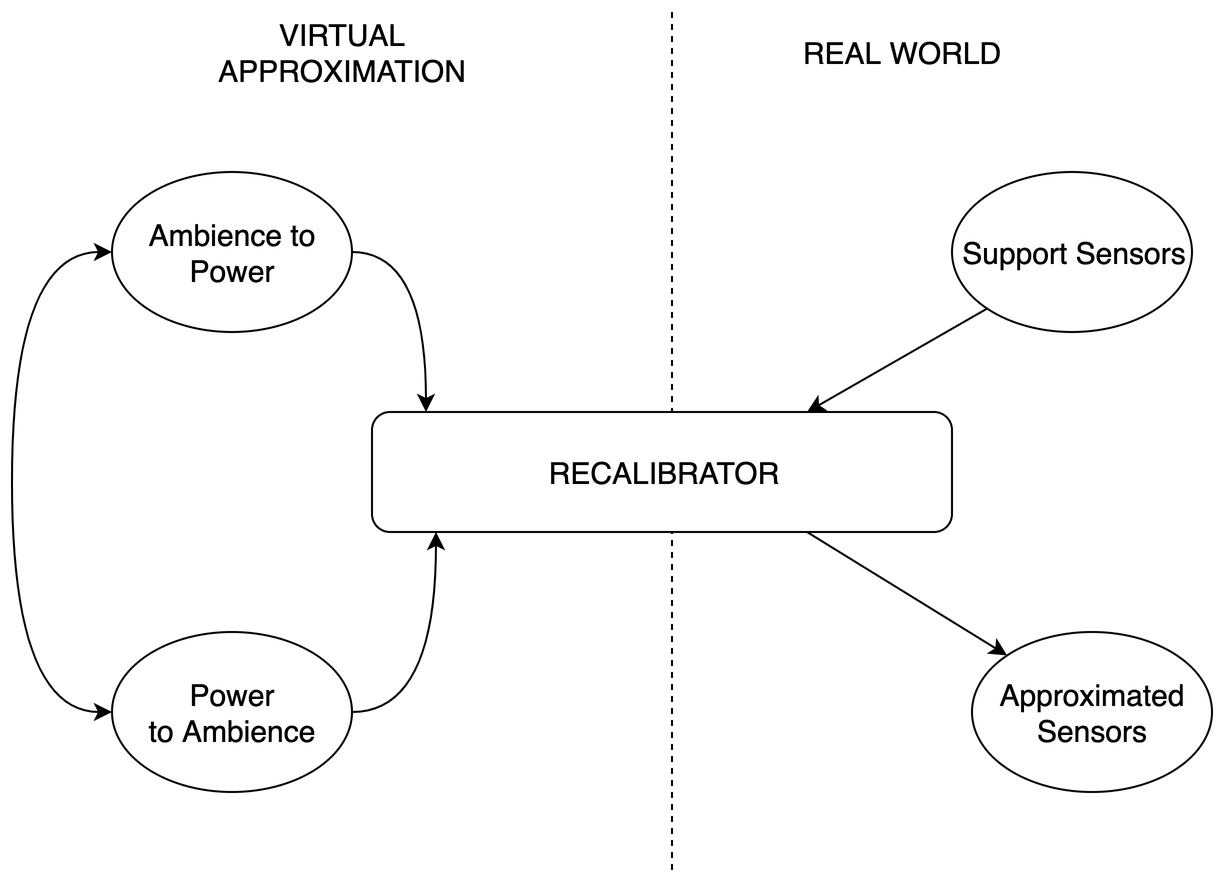
\includegraphics[width= 7cm]{img/schematicBlock.png}
    \caption{Schematic Representation of System Components}
    \label{fig:schematicBlock}
\end{figure}




The  smart building stack for online learning comprises of 2 components that can toggle between learning and deployment modes. 
The motivation behind the system design is to explore the potential of deep learning through organizing functional blocks that can enable multiple task performances to improve in an isolated manner or benefit from joint training.

\begin{itemize}
\item Ambience to Power Inverter projects the temperature and  luminosity values from sensors into the policy space that controls HVAC and illumination power respectively for example.
\item Power Predictor layer is a control policy layer that learns the control signals from temperature and luminosity encoding in a single task learning mode. In multi task mode, it additionally learns to optimize what are the minimum set of sensors that we need to install and where without degrading the performance too much ($ < 10\%$). 
 
\item Power To Ambience Translator expresses the effect of control signals on ambient sensor values. Fie example, if the HVAC power is low, will that mean the temperature will rise to equilibrium with the outdoor.  The output of this layer are approximating models that explains the cause-effect between ambience value approximate from predicted control points. 
\item Forecasting Modules act on a single channel by predicting for next $K_a$ time steps ahead with $K_b$ look backs. We introduce this model with an intention to replace a sensor with its forecasting counterpart and reduce the sensor capital cost to 0 ideally, 
\end{itemize}



data-set is split into k fold partitions namely and the linear model is learned leaving out one partition. 
However in an online fashion, the model is retrained on historic data starting from time $t_0$ till time $t$.
Its performance is evaluated during the test period before switching back to train mode. 


For each channel, the single task for the system is learn to predict power consumption from the stream of sensors values. 
We want to explain the interaction between the dependent and independent variables with significant values under single and multiple channel input settings.

\begin{figure}%
    \centering
    \subfloat[\centering Training Predictions ]{{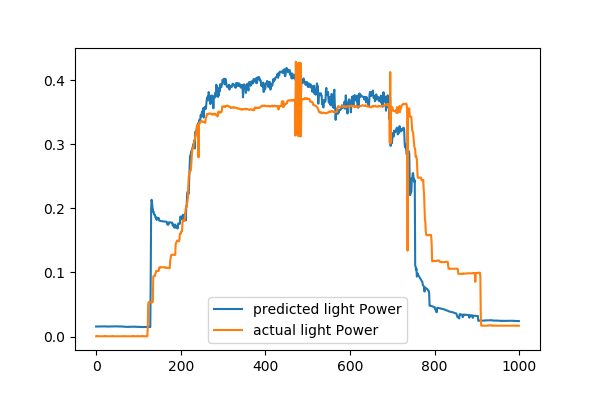
\includegraphics[width=0.47\textwidth]{img/lassocv-lighttrain.png} }}%
    \qquad
    \subfloat[\centering Testing Predictions ]{{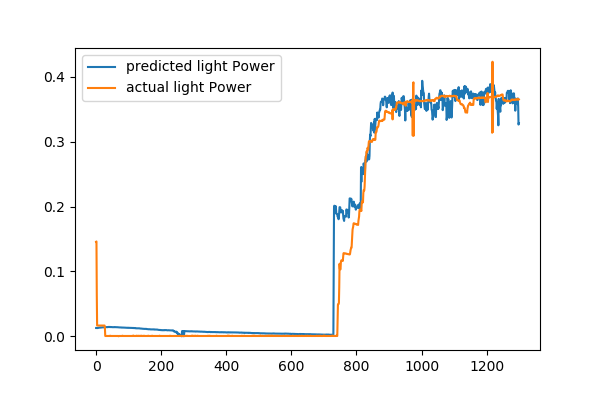
\includegraphics[width=0.47\textwidth]{img/lassocv-lighttest.png} }}%
    \caption{Approximating Illumination power from ambient sensors [luminosity, humidity and temperature] by a Cross Validated Lasso Regression Model  }%
    \label{fig:ambient2lightpower}%
\end{figure}



\section{NGIS Implementation}
\label{implem}
This section presents the implementation details of NGIS, the software we developped to enhance the existing Qarnot's smart building platform.
We first describe how IFC (Industry Foundation Classes) files are parsed to generate a spatio-temporal graph as detailed in the deliverable $D4.2$. We then present the architecture of the building management software along with the different APIs (Application Programming Interface) and configuration settings. Finally, we end this section by benchmarking the average runtime of all back-end routines to assess the effectiveness of our implementation.

\subsection{Building Information Parsing}

 %(language, lines of code, maybe class diagram or stuff like that... ), how does it run , how long does it take to run, etc 


\begin{figure}
    \centering
    \includegraphics[width=0.95\textwidth]{img/ifcParserClassDiagram.jpg}
    \caption{Class Diagram of IFC Parser}
    \label{fig:ifcParserClassDiagram}
\end{figure}
 
 The first part of the software deals with information extraction from an IFC file. We define 2 principal classes (QPRODUCT and Q3DPARSER) to absorb the information defined in a building modelling file. QPRODUCT has a attribute named \textit{globalID} to store the BIM (Building Information Modeling) identifier, along with \textit{type of Product}. An instance of the 3D parsing class stores multiple cross-sections of a building element on horizontal and vertical planes. Class functions \textit{returnHullPolygon} and \textit{getBoundingBox} return a list of 3D coordinates at a height denoting a convex hull or the bounding box of the building element. Doors, spaces, storeys, windows, walls and stairs are encapsulated as derived classes of QPRODUCT and Q3DPARSER. Finally all building elements are referenced through a class called QBUILDING which stores the topological connectivity graph and hash-map of building metadata referenced by the global identifier. Figure \ref{fig:ifcParserClassDiagram} shows the UML diagram of the classes. The software is made available and can be pulled from Docker hub by imagename: \textit{angmit/ifcparser:v2.0}. The parser allows  to specify an input IFC file, store the computed results, specify hull formation or graph generation and reload an intermediate output. Its usage is as follows:

\newpage
\begin{lstlisting}
  usage: parser.py [-h] [-i INPUT_FILE] [-o OUTPUT_DIR] [-r RELOAD] 
  [-g GRAPH_GEN] [-u HULL_GEN] [-f FLOORPLAN_GEN]
optional arguments:
-h, --help            show this help message and exit
-i, --input_file : path of the ifc file.
-o, --output_dir : path of the output directory.
-r, --reload : True reloads a previous computation specified by output dir.
-g, --graph_gen : True to generate a topological graph
-u, --hull_gen : True to compute a hull
-f, --floorplan_gen : True to generate floorplans storeywise
-e, --EPS : Buffer margin as a float for hull computation
\end{lstlisting}


\subsection{Building Management Software }
The Building Management Software is implemented via 4 dockers containers as described in Figure~\ref{fig:yaml_bms}. They provide the following services:
\begin{itemize}
    \item Qfrontend is pythonic frontend built using Streamlit Framework and made available under the Docker-image name "angmit/oasisfrontend:v2.2". The front-end sends http requests to a back-end server known as the Qapi-service.
    \item Qapi-service is a REST server whose API (Application Programming Interface) routes are enlisted in Table \ref{table:apilist}. The flask application listens on port 5001 which is mapped to http port 80 for replying to incoming web-requests.   
    \item Qlearning-service is invoked periodically and executes a set of routines that analyze incoming data, predict semantic activities, save the insights on to a database for the building.
    \item Qinfluxdb  is a time-series database which stores ambient sensor measurements, electrical power readings and derived insights. The machine learning models are stored on S3 bucket in the Qarnot Compute platform.
\end{itemize}
\begin{figure}[h!]
     \centering
     \subfloat[][YAML specification (part 1)]{\includegraphics[width= 0.45\linewidth]{./img/Yaml_BMS1.png}  }
     \subfloat[][YAML specification (part 2) ]{\includegraphics[width= 0.45\linewidth]{./img/Yaml_BMS2.png} }
      \caption{Example of YAML configuration file to deploy the $4$ containers underlying the Building Management Software.}%
    \label{fig:yaml_bms}%
\end{figure}






% Please add the following required packages to your document preamble:
% \usepackage{booktabs}
\begin{table}[]
\begin{tabular}{@{}|l|l|@{}}
\toprule
Route                                & Argument     \\ \midrule
/v1/get-raw-data                   & config-file, start-time, end-time  \\ \midrule
/v1/get-oracle-detection           & config-file, start-time, end-time                                              \\ \midrule
/v1/guess-appliances                & config-file, start-time, end-time                                              \\ \midrule
/v1/running-appliances              & config-file, start-time, end-time                                              \\ \midrule
/v1/train-forecast-channel         & config-file, start-time, end-time, modelSavePath, column, sensor               \\ \midrule
/v1/predict-forecast-channel       & modelSavePath, start-time, lookAheadIntervals                                    \\ \midrule
/v1/get-room-status                & config-file, start-time, end-time                                              \\ \midrule
/v1/get-air-quality                & config-file, start-time, end-time                                              \\ \midrule
/v1/get-energy-metadata            & config-file, start-time, end-time                                              \\ \midrule
/v1/fetch-calendar-events          & config-file, start-time, end-time                                              \\ \midrule
/v1/get-waste-energy               & config-file, start-time, end-time                                              \\ \midrule
/v1/spatial-navigation              & sourceID, targetID                                                                \\ \midrule
/v1/get-storeys                     &                                                                                   \\ \midrule
/v1/building-metadata               &                                                                                   \\ \midrule
/v1/show-floorplan                  & storeyID                                                                          \\ \midrule
/v1/get-live-weather               &                                                                                   \\ \midrule
/v1/get-daily-weatherdata          & day                                                                               \\ \midrule
/v1/predict-learner                 & start-time, end-time, model-name,  config-file, outputPath                    \\ \midrule
/v1/train-multi-column-forecast   & config-file,  scalerSavePath,  modelSavePath,  trainOutputPath                   \\ \midrule
/v1/predict-multi-column-forecast & config-file, scalerSavePath,  modelSavePath,  testOutputPath                     \\ \midrule
/v1/train-learner                   & config-file, scalerSavePath,  modelSavePath,  trainOutputPath, inferencePath     \\ \midrule
/v1/federated-learning              & config-file, scalerSavePath,  modelSavePath,  trainOutputPath, inferencePath     \\ \midrule
/v1/ventilation-suggestions     & config-file, start-time, end-time  \\ \bottomrule
\end{tabular}
\caption{REST API list}
\label{table:apilist}
\end{table}


 Sensor equipped space configurations are specified in a YAML format (see Figure~\ref{fig:yaml_sensor}). The config file specifies an object denoted by \textbf{spaces} where multiple spaces can be enlisted by their name and inside each space, devices are registered with their type and access identifier. The ambient information comprises of humidity, temperature, sound, light, and carbon dioxide (CO$_2$) coming from sensors distributed across rooms. Below is a sample of a meeting room, with a Qrad and private office having a Netatmo sensor recording the above-mentioned channels to the Qinflux-db at a \textbf{resolution} of 5 minutes.

\begin{figure}[h!]
     \centering
     \subfloat[][YAML specification (part 1)]{\includegraphics[width= 0.30\linewidth]{./img/Yaml_sensor1.png}  }
     \subfloat[][YAML specification (part 2) ]{\includegraphics[width= 0.30\linewidth]{./img/Yaml_sensor2.png} }
      \caption{Example of YAML configuration to specify the sensors configuration}%
    \label{fig:yaml_sensor}%
\end{figure}


Electrical power is measured across a supply line catering to multiple sockets or appliances or illumination needs. An energy-meter (\textit{Schneider eco-compteur}) records the power consumption required for the cuisine, heating services, sockets and lightnings  (See Figure~\ref{fig:yaml_elec}). The minimum and maximum power cap reading is from 0.001 to 150 Kilo-watt.
\begin{figure}[h!]
     \centering
     \subfloat[][YAML specification (part 1)]{\includegraphics[width= 0.38\linewidth]{./img/Yaml_elec1.png}  }
     \subfloat[][YAML specification (part 2) ]{\includegraphics[width= 0.38\linewidth]{./img/Yaml_elec2.png} }
      \caption{Example of YAML configuration to specify the power consumption monitoring}%
    \label{fig:yaml_elec}%
\end{figure}

Inside the docker image \textit{angmit/oasisbackend:v2.3}, the code is organised into 7 pythonic class modules as shown in Figure \ref{fig:oasisClassDiagram} that are responsible for storing the building data, utilising spatial orientation for navigation, ventilation, fetching sensor plus weather data, aggregating calendar events, generate automatic insights about room occupancy, illumination status, CO$_2$ dissipation suggestions and energy savings. The Qapi-service exposes certain endpoints of the classes via the Flask Application as stated in Table \ref{table:apilist}. 
\begin{figure}[h!]
    \centering
    \includegraphics[width=\textwidth]{img/oasisClassDiagrams.jpg}
    \caption{Class Diagram of Back-end }
    \label{fig:oasisClassDiagram}
\end{figure}


\subsection{Run-times}

 
\begin{table}[]
\begin{tabular}{|l|l|l|}
\hline
Route                             & Task Caller                     & Average Run-time (seconds) \\ \hline
/v1/get-raw-data                  & Qlearning-service, Qapi-service & 87 $\pm$ 23                \\ \hline
/v1/get-oracle-detection          & Qlearning-service               & 10 $\pm$ 6                 \\ \hline
/v1/guess-appliances              & Qlearning-service               & 360 $\pm$ 10               \\ \hline
/v1/running-appliances            & Qlearning-service               & 500 $\pm$ 49               \\ \hline
/v1/train-forecast-channel        & Qlearning-service               & 400 $\pm$ 34               \\ \hline
/v1/predict-forecast-channel      & Qapi-service                    & 9 $\pm$ 2                  \\ \hline
/v1/get-room-status               & Qapi-service                    & \textless 1 second         \\ \hline
/v1/get-air-quality               & Qapi-service                    & \textless 1 second         \\ \hline
/v1/get-energy-metadata           & Qapi-service                    & \textless 1 second         \\ \hline
/v1/fetch-calendar-events         & Qlearning-service               & 1-2 seconds                \\ \hline
/v1/get-waste-energy              & Qapi-service                    & \textless 1 second         \\ \hline
/v1/spatial-navigation            & Qapi-service                    & \textless 1 second         \\ \hline
/v1/get-storeys                   & Qapi-service                    & \textless 1 second         \\ \hline
/v1/building-metadata             & Qapi-service                    & \textless 1 second         \\ \hline
/v1/show-floorplan                & Qapi-service                    & \textless 1 second         \\ \hline
/v1/get-live-weather              & Qapi-service                    & \textless 2 seconds        \\ \hline
/v1/get-daily-weatherdata         & Qlearning-service               & 7 $\pm$ 3                  \\ \hline
/v1/predict-learner               & Qapi-service                    & \textless 10 seconds       \\ \hline
/v1/train-multi-column-forecast   & Qapi-service                    & 600-800 seconds            \\ \hline
/v1/predict-multi-column-forecast & Qapi-service                    & \textless 10 seconds       \\ \hline
/v1/train-learner                 & Qlearning-service               & 670 $\pm$ 8                \\ \hline
/v1/federated-learning            & Qapi-service                    & 550 $\pm$ 34               \\ \hline
/v1/ventilation-suggestions       & Qlearning-service               & 130 $\pm$ 3                \\ \hline
\end{tabular}
\caption{Average Run Times of Back-end Routines }
\label{table:runtimes}
\end{table}

We observe a range of run-times from a few seconds to up to 15 minutes for tasks catering to data fetching, inference generation and learning. In Table \ref{table:runtimes}, we present the average execution time taken by API routines over 10 random runs and also highlight the calling function (\textit{Task Caller}). The volume of sensor data fetched can range from 5 minutes to 7 days and is proportional to the look-back interval. The maximum run time reported is for $24 \times 7 \times 288 = 48384$ data samples, with each data sample having at most 5 features for ambience plus 4 for energy reading. We observe that the inference tasks generally take less than 10 seconds while the training tasks can last from 7-15 minutes. During an inference task, the software downloads the latest version of a machine-learnt model from Qarnot's S3 bucket, reads the input data, returns the inference and deletes the model from local memory.

\newpage
\section{NGIS Applications}
\label{applications}
NGIS has been developed to tackle various uses cases related to the energy consumption in smart buildings.
In fine, the goal is to reduce the overall energy consumption in buildings as it is becoming mandatory to reduce their footprint by 40 $\%$ by 2030, towards -60 $\%$ in 2050. To this end, we present numerous examples of NGIS applications in the following sections.


\subsection{Spatio-Temporal Activity Graph (STAG)}
This section describes how NGIS leverages building geometry and spatial orientation to provide ambient intelligence.
\begin{figure}[t!]
\centering
\subfloat[Experimental Setup Framework of Qarnot's building. \\ $3$ rooms are circled in red (namely Babbage, Lunch and Jacquard).\label{fig:qarnot_plan}]{\includegraphics[width=0.49\textwidth]{img/QarnotExperiment.png}}\hfill
\subfloat[The associated Spatio-Temporal Activity Graph.\label{fig:activitygraph}]{\includegraphics[ width=0.49\textwidth]{img/activitygraph.png}}
\caption{Qarnot's building setup}
\end{figure} 
 Availability of raw sensor data often makes it possible to detect temporal activities that are distributed over space. Often specific activities are related to a spatio-temporal dynamism amongst multiple spaces. We intend to capture the causality-effect relationship by defining a
{Spatial Graph $\mathcal{G}$ } that represents connectivity amongst building elements. Formally, at any cutting plane $\Xi$, $\mathcal{G}( \Xi)$ will be a set of building elements as nodes and connectivity links as edges.

$$  \mathcal{G}( \Xi) =\{  <e, \mathcal{N}_2(e, \Xi) > | e \in \mathcal{B}\} $$
where $\mathcal{N}_2$ is the neighbourhood operator described more thoroughly in the Deliverable $D4.2$. 
 

The utility value of a spatial graph is to understand information flow of ambient sensor signals like CO$_2$, humidity, temperature, noise and luminosity between interconnected spaces. As an example, we point out to Fig.~\ref{fig:qarnot_plan}, where we have circled out three rooms in red, each specifying different spatial profiles.  The corresponding spatial graph view when superimposed with the distribution of signals and states of doors and windows yields a Spatio Temporal Activity Graph as shown in Fig. \ref{fig:activitygraph}.  Notice that  circle to the right encircles a kitchen-space named "Babyfoot" and is without windows, and is instead connected to a common space and two other spaces via a door.  The room in the middle named "Babbage" is a room intended for meeting purposes without any windows but a single door. The circle at the left is a room, "Jacquard" with two doors and a window, with one of the doors connecting to the common space. Figure~\ref{fig:wall} shows the walls attached to spaces on a floor-plan, while Figure~\ref{fig:spaces} depicts the space contours.
 


We aim to answer how are sensor signals distributed, precisely we want to have a deep understanding of the link between space and signal dispersion. We can not expect every room, door, window to have ambient or contact sensors. Thus in a $STAG$, there will be nodes with no information. There can be two cases that follows:

\begin{itemize}
\item  The no information zone imparts little or no knowledge to our region of interest in the graph, for instance "Space 1" or "Space 2" in Fig: \ref{fig:activitygraph} which may be usually unused.
\item The nature of information needs to interpolated from the data points surrounding our region of interest, for instance "Common Space" in Fig: \ref{fig:activitygraph}. Notice that an activity like talking in the common space can trigger a change in sensor values in the room "Jacquard" if the doors are open and may declassify the room from being "idle" to "occupied". 
\end{itemize}

\textbf{Pruning nodes of no/little interest}


Let us start with a space that do not have any sensors attached to them, thus being a blind spot. If such a blind spot is connected with doors and windows that do not have any sensors attached to it, we drop the blind spots from the graph. However if such a blind spot interconnects two or more spaces with sensor signals attached, we retain the node of the graph for instance if "Space 1" in Fig. \ref{fig:activitygraph} does not have a door sensor, it can be dropped since it does not interconnect two spaces. The information coverage algorithm (described in Section $2.3$ of the deliverable $D4.2$) uses depth first search to return information coverage for a building element by listing nearby elements with sensor data sources. Data coming from $i^{th}$ sensor -equipped building element is represented as $D^i$ and total data is D = $\cup D^i $ $\forall i$. In real life setting often data labelling of $y$ is absent and thus certain heuristics are applied to approximate the solution of a problem. 
%  \subsection{Colour Coding }
 
%  We apply the following colour convention to label our nodes and we will refer by the colour when processing information flow through them. 
% \begin{itemize}
% \item  If a blind spot is not deleted from STAG, then it is colour coded "black.
% \item  Spaces with sensors are coded "Blue"
% \item  Doors and windows with sensors are coded "red" and "green" respectively.
% \end{itemize}

% Applying the convention to the our model and assuming absence of sensors in "Space 1,2,3 and Common Space", Fig \ref{fig:activitygraph} gets transformed into Fig: \ref{fig:prunedactivitygraph}.
 
% \begin{figure}[H]
% \centering
%   \includegraphics[width=0.70\linewidth]{img/prunedactivitygraph.png}
%   \caption{Pruned Activity Graph   }
%   \label{fig:prunedactivitygraph}
% \end{figure}



\begin{figure}
     \centering
     \subfloat[][Wall Boundaries (red) \label{fig:wall}]{\includegraphics[width= 0.5\linewidth]{./img/wallHighlight.png}  }
     \subfloat[][Space Contours (green) \label{fig:spaces}]{\includegraphics[width= 0.5\linewidth]{./img/spaceHighlight.png} }
      \caption{ Walls and Space highlights parsed from IFC file. }%
    \label{fig:wallSpaceHighlights}%
\end{figure}
\begin{figure}
     \centering
     \subfloat[][Doors (red)]{\includegraphics[width= 0.5\linewidth]{./img/doorHighlight.png}  }
     \subfloat[][Windows (green) ]{\includegraphics[width= 0.5\linewidth]{./img/windowHighlight.png} }
      \caption{ Highlighting ventilation Sources (door, window) post parsing from IFC file. }%
    \label{fig:ventilationHighlights}%
\end{figure}

\subsection{Virtual CO$_2$ sensors}

\begin{figure}
     \centering
     %\subfloat[][Location of CO$_2$ sensors in rooms circled with red.]{\includegraphics[width= 0.5\linewidth]{./img/QarnotExperiment.png} \label{fig:qe} }
     %\subfloat[][]
     {\includegraphics[width= 0.8\linewidth]{./img/virtualco2.png} }
      \caption{Ventilation graph: connecting sensor enabled spaces (green) and without sensed spaces (red)}%
    \label{fig:virtualco2}%
\end{figure}

Air quality management is rudimentary for ensuring indoor comfort and sound health of people. Figure \ref{fig:ventilationHighlights} highlights the doors and windows on a floorplan. Existing literature relies on temperature and humidity as a metric of comfort. Concerning health, CO$_2$ is primarily measured (shown in Table \ref{table:co2Values}) followed by Volatile organic compounds (VOC) and Particulate Matter (PM). We observe that air circulation pathways through spaces, doors or windows change in accordance with closing or opening of a door/window. Although people rely on sensors and active appliances to monitor their air quality, taking actions to alter IAQ (Indoor Air Quality) is non trivial. To help our cause, we approximate gas diffusion models in a building with $CO_2$ build up and dissipation rates across connected spaces. For example, we want to know if at any instant the cafeteria records 1000 ppm of CO$_2$, what is the optimal ventilation route and how much time is required to bring down IAQ to acceptable levels.

\begin{table}[h!]
\centering
\begin{tabular}{|l|l|}
\hline
Air Quality & CO$_2$ Level          \\ \hline
Excellent   & $\leq$400 ppm         \\ \hline
Average     & 400-600 ppm           \\ \hline
Moderate    & 600-1000 ppm          \\ \hline
Poor        & $\geq$  1000 ppm \\ \hline
\end{tabular}
\caption{Relation between CO$_2$ levels and classes of Air Quality}
\label{table:co2Values}
\end{table}
 
The CO$_2$ mass balance equation \cite{cali2015co2} of a room of volume $V_{room}$ with $n_{occ}$ occupants, each with $C_{occ}$ carbon dioxide production rate per person  \cite{persily2017new} present in a room exchanging $\Dot{m_{vent}}$ air mass at a concentration difference of $(C_{room} - C_{space})$ is given by 

\begin{equation}
    V_{room} \frac{\delta C_{room}}{\delta t} = n_{occ}C_{occ} + \Dot{m}_{vent} ( C_{vent} - C_{room})
    \label{eq:mass_balance}
\end{equation}
 
With discrete CO$_2$ readings at $R_{sensor}$ resolution(mins), 
\begin{equation}
    \frac{\delta C_{room}}{\delta t} \approx \frac{C^{t+1}_R - C^t_R}{\Delta R_{sensor}}
    \label{eq:discreteco2}
\end{equation} 

Let $E_s, E_w, E_d$ be the set of elements connected directly to a room (R) with CO$_2$ readings at time t given by $C_R^t$. Air mass exchange through doors and windows is proportional to the concentration difference between the room and adjacent spaces. Thus combining Equations \ref{eq:mass_balance} and \ref{eq:discreteco2}, we formulate the graph based representation of air circulation as :
\begin{equation}
V_{room} \frac{C^{t+1}_R - C^t_R}{\Delta R_{sensor}} = n_{occ}C_{occ} + \Sigma_{z \in \{E_w, E_d\}} \Sigma_{y \in Neighbour(z), y \neq R} (C_{R} - C_y){m_{z,R}} + \Sigma_{y \in \{E_s\}} (C_{R} - C_y){m_{y,R}}
\label{eq:co2distribution}
\end{equation}
where $m_{x,R}$ represents permeability co-efficient of air exchange between room (R) and connector $x$.  To estimate the steady state having $n_{occ}$ occupants, according to equation \ref{eq:co2distribution}, the  CO$_2$ concentration at every connected space needs to be known. Placing sensors at every space maybe infeasible or expensive and instead, partial information may be available. For example, Fig. \ref{fig:qarnot_plan} shows such a data collection scenario from 3 rooms namely kitchen ($R_K$), meeting room ($R_M$), and a private cabin ($R_C$). Our first contribution in IAQ is to estimate CO$_2$ levels at adjacent spaces leveraging the connectivity graph, followed by prediction of number of occupants. The occupancy count coming from analysing structural CO$_2$ data is stored as a fact $(t, n_{occ}^t, location = R )$, where $t$ is the timestamp of the observation. 



\begin{figure}
     \centering
     \subfloat[][ \\ Estimating CO$_2$ in a passage (in yellow). \label{fig:passage}]{ \includegraphics[width=0.49\linewidth]{img/passage.png} }
     \subfloat[][Ventilation Graph View from Kitchen.\label{fig:ventilationPath} ]{\includegraphics[width=0.49\linewidth]{img/ventilationPath.png}}
      \caption{Air quality (left) and Ventilation graph (right) examples.}%
\end{figure}


The ventilation graph illustrated in Fig \ref{fig:virtualco2}, concerning 3 rooms $(R_K,R_M,R_C) $ is connected to a common passage $R_P$. Passage is devoid of sensors and hence want to estimate the CO$_2$ estimation by the following set of equations:

\begin{equation}
    V_{K} \frac{C^{t+1}_K - C^t_K}{\Delta R_{sensor}} = n_{K}C_{occ} +  (C_P^t - C_K^t){m_{K,P}}
    \label{eq:co2kitchen2passage}
\end{equation}
\begin{equation}
V_{M} \frac{C^{t+1}_M - C^t_M}{\Delta R_{sensor}} = n_{M}C_{occ} +  (C_{P}^t - C_M^t){m_{M,P}}
\label{eq:co2babbage2passage}
\end{equation}
\begin{equation}
V_{C} \frac{C^{t+1}_C - C^t_C}{\Delta R_{sensor}} = n_{C}C_{occ} +  (C_{P}^t - C_C^t){m_{C,P}}
\label{eq:co2cabin2passage}
\end{equation}


 The analytical solution for estimating CO$_2$ concentration in the passage is given by 

\begin{equation}
    C^t_p = C^t_X + \frac{1}{m_{X,P}} (V_i \frac{C^{t+1}_X - C^t_X}{\Delta R_{sensor}} - n_X C_{occ} )
\end{equation}
, where $X \in \{K, M, C \}$. The permeability coefficient $m_{x,P}$ is proportional to the cross-sectional area of a door or window ($x$) connected to space $P$ and ranges from [0,1] depending if the object is closed or opened respectively. We adopt a two pronged strategy to approximate $m_{x,P}$. 
\begin{itemize}
    \item Using the semantics of our data set we know that there usually are no occupants during non-office hours (20h - 07h (+1 day)), except for party dates. CO$_2$ data during this period is utilised to approximate the value of $m_{x,P}$.
    \item During office hours, we assume that activities are performed in closed spaces and hence the coefficient is reduced when occupant is detected. 
\end{itemize}





In Figure \ref{fig:ventilationPath}, we illustrate a use-case of ventilation graph to predict dissipation of CO$_2$ build up from a space like kitchen. We highlight  6 paths connected to outdoor environment via windows (in blue) and 2 spaces adjacent to kitchen: a common passage (in red), reception (in yellow).  Now one of the suggestions can be to open the window of the private office room, but if there is an ongoing meeting, such an action may not be feasible. Knowledge or a priori belief about semantic usage of a space is built from activity monitoring that predicts either occupancy count or zones of activity. In Figure \ref{fig:co2Variation}, we show show a 24 hour CO$2$ profile of the three rooms under monitoring a kitchen, meeting room and private office connected to a common passage as shown in Figure \ref{fig:passage}.




\begin{figure}
     \centering
     \subfloat[][ CO$_2$ sensor values distribution on a working day ]{\includegraphics[width= 0.5\linewidth]{./img/freq_babbage.png} \label{fig:freq_babbage} }
     \subfloat[][ Discrete Time Differential at 5 minute resolution  ]{\includegraphics[width= 0.5\linewidth]{./img/diffCO2.png} \label{fig:diffCO2}}
     \\
     \subfloat[][ CO$_2$ sensor values distribution on the same day ]{\includegraphics[width= 0.5\linewidth]{./img/freq_kitchen.png} \label{fig:freq_kitchen} }
     \subfloat[][ Discrete Time Differential at 5 minute resolution  ]{\includegraphics[width= 0.5\linewidth]{./img/freq_kitchen_diff.png} \label{fig:freq_kitchen_diff}}
     \\
     \subfloat[][ CO$_2$ sensor values distribution from the window enabled private office  ]{\includegraphics[width= 0.5\linewidth]{./img/jacquard_co2.png} \label{fig:jacquard_co2} }
     \subfloat[][ Discrete Time Differential at 5 minute resolution  ]{\includegraphics[width= 0.5\linewidth]{./img/freq_jacquard_diff.png} \label{fig:freq_jacquard_diff}}
      \caption{CO$_2$ Profiling}%
    \label{fig:co2Variation}%
\end{figure}

\subsection{Augmented Reality}
 
We enrich the building information representation by incorporating static objects that govern the semantic usage of a space. For example, presence of a coffee machine will make people arrive at that spot to brew a cup of coffee with an energy dissipation proportionate to the run-time of the device. The work aims at embedding a layer of augmented reality and deriving rules or implement policies that can lead to potential energy saving or in-house comfort management. Privacy concerns restrict all places to be put under video-surveillance. So to enrich a space, we create a virtual view derived from multiple images. The target is to enhance the semantics of a space with the spatial distribution of tables, chairs, overhead tube-lights, bulbs and other electrical appliances. The intuition behind such an approach is that human activities are concentrated in regions where there are objects of interest and most likely to form the zones of energy dissipation footprints. 

We want to approximate the semantic utility of space from electrical appliances, lights, furniture  arrangements. For a set of images in a room, we extract the following features.
\begin{itemize}
    \item \textbf{Illumination Coverage} is computed to detect the sources of illumination like over head tube-lights, desktop lights, or bulbs and estimate the position of pre-installed lighting loads in a space. We overlay the contour of the detected object on top of the space. Each object is a contained in a rectangular bounding box represented by two diagonally opposite vertices and a semantically segmented image mask.  
    
    \item \textbf{Furniture Placement} is a layer to detect natural grouping of human occupancy in a space by extracting and analyzing how are chairs and tables are organized from multiple image views. This feature is useful for the system to auto setup rules regarding energy savings, air quality or comfort maintenance by correlating spatial distribution with activity detection.  
    
    \item \textbf{Energy Hot-spots} are defined as spots in a building where non-illumination electrical loads are situated. The commonly available energy dissipation points in a building are wall-sockets, electrical appliances like fridge, oven, dishwasher, washing machine, laptop chargers, desktop monitors. Thus we construct an energy profiling of a space with a target to deliver non-intrusive spatial disintegration of electrical power consumption. 
\end{itemize}


For the image classification task, we utilize the state of the art deep learning models, that comes pre-trained classes. For custom object detection, we train a single shot detector like YOu-Look-Once (YOLO V5) \cite{glenn2021yolov5} after annotating the images using a open source annotation tool (LabelMe). To increase the data set size, we perform image augmentation using the python library \textit{Albumentation} \cite{buslaev2018albumentation} by altering the rotation, scale, hue and saturation. We add spatio-semantic features like spatial connection, illumination, tables and chairs to enrich a space for deriving semantic activities as shown in Table \ref{table:semanticSpace}.  

\begin{figure}
    \centering
    \includegraphics[width=\linewidth]{img/Developpeurs.png}
    \caption{Top view of an office space with 5 groups in table (purple) and overhead lights (green)}
    \label{fig:Developpeurs}
\end{figure}


\begin{figure}
     \centering
     \subfloat[][Furniture Placement]{\includegraphics[width= 0.5\linewidth]{./img/Developpeurs-tables.png}  }
     \subfloat[][Illumination Coverage]{\includegraphics[width= 0.5\linewidth]{./img/Developpeurs-lights.png} }
      \caption{Extraction of Illumination Coverage and Furniture Placement from a room (Fig. \ref{fig:Developpeurs}) snapshot.}%
    \label{fig:Developpeurs-features}%
\end{figure}

 
 
 \begin{table}[]
\begin{tabular}{|l|l|l|l|l|}
\hline
Space Name           & Illumination             & Tables + Chairs                                                                                                        & Semantic Activity         & Spatial Connections        \\ \hline
Developers   & 5 overhead        & \begin{tabular}[c]{@{}l@{}}5 sub groups\\ 16 person capacity\end{tabular}                                              & Working, Idle             & 1 doors, 1 window, 1 Space \\ \hline
Marketing     & 4 lights                 & \begin{tabular}[c]{@{}l@{}}3 sub groups\\ 10 person capacity\end{tabular}                                              & Working, Idle             & 2 doors, 1 window, 1 Space \\ \hline
4MTEC             & 1 light                  & 6 person capacity                                                                                                      & Working, Idle             & 2 Doors, 1 Window          \\ \hline
Babbage           & 1 light                  & 5 seater capacity                                                                                                      & Meeting, Idle             & 1 Door                     \\ \hline
Jacquard  & 1 light                  & 5 seater capacity                                                                                                      & Meeting, Private Office   & 1 Window, 1 Door           \\ \hline
Cuisine           & Multiple  & \begin{tabular}[c]{@{}l@{}}12 seater table\\ 4 seater sofa\\ 4 seater meeting table\\ 2-4 player Babyfoot\end{tabular} & Eating, Working, Partying & 1 Passage, 2 Doors         \\ \hline
Accueil           & 2 lights                 & (2 + 1+3) seater capacity                                                                                              & Reception                 & 1 Door, 1 Window           \\ \hline
\end{tabular}
\caption{Extraction of Rooms of Interest based on semantic and structural ontology. }
\label{table:semanticSpace}
\end{table}
 
 
 
\newpage
\subsection{Lux Estimator}
\begin{center}
\begin{table}[]
 \centering 
\begin{tabular}{ll}
\hline
\multicolumn{1}{c}{\textbf{Illuminance (lux)}} & \textbf{Surfaces illuminated by}                                            \\ \hline
\multicolumn{1}{|l|}{0.0001}                   & \multicolumn{1}{l|}{Moonless, overcast night sky (starlight)}               \\ \hline
\multicolumn{1}{|l|}{0.002}                    & \multicolumn{1}{l|}{Moonless clear night sky with airglow}                  \\ \hline
\multicolumn{1}{|l|}{0.05–0.3}                 & \multicolumn{1}{l|}{Full moon on a clear night}                             \\ \hline
\multicolumn{1}{|l|}{3.4}                      & \multicolumn{1}{l|}{Dark limit of civil twilight under a clear sky}         \\ \hline
\multicolumn{1}{|l|}{20–50}                    & \multicolumn{1}{l|}{Public areas with dark surroundings}                    \\ \hline
\multicolumn{1}{|l|}{50}                       & \multicolumn{1}{l|}{Family living room lights}
\\ \hline
\multicolumn{1}{|l|}{80}                       & \multicolumn{1}{l|}{Office building hallway/toilet lighting } \\ \hline
\multicolumn{1}{|l|}{100}                      & \multicolumn{1}{l|}{Very dark overcast day }                          \\ \hline
\multicolumn{1}{|l|}{150}                      & \multicolumn{1}{l|}{Train station platforms }                        \\ \hline
\multicolumn{1}{|l|}{320–500}                  & \multicolumn{1}{l|}{Office lighting }         \\ \hline
\multicolumn{1}{|l|}{400}                      & \multicolumn{1}{l|}{Sunrise or sunset on a clear day.}                      \\ \hline
\multicolumn{1}{|l|}{1000}                     & \multicolumn{1}{l|}{Overcast day }        \\ \hline
\multicolumn{1}{|l|}{10,000–25,000}            & \multicolumn{1}{l|}{Full daylight (not direct sun) }                  \\ \hline
32,000–100,000                                 & Direct sunlight                                                             \\ \hline
\end{tabular}
\caption{Variation of illumination intensity on a building with respect to weather conditions. }
\label{table:luxVariation}
\end{table}
\end{center}

\begin{figure}
\centering
  \includegraphics[width=0.5\linewidth]{./img/illuminationEffect.png}
  \caption{ Direct naturally illuminated space (in yellow) and shared window connections with 6 different spaces (in red) and 1 sensor placed (in bright pink) on Qarnot's office floor-plan. }
  \label{fig:illuminationEffect}
\end{figure}

Energy is wasted if lights are switched on where no physical activity is ongoing or there are unwanted illumination. Typically in an office or household setting, \textbf{Illumination Coverage} is organized around either \textbf{Furniture Placements} or \textbf{Energy Hotspots}. The functionality is designed to compute reactive illumination control for a space taking into account the occupancy status, absence or presence of a sun-lit window, and natural activity groupings. For the sake of simplicity, we assume every illumination source as a point object placed in a non-reflecting space. The location of the source ($S_i$) is given by the 3D centroid of it's corresponding bounding box. The law of light propagation \cite{voudoukis2017inverse} states that the intensity ($\mathcal{I}$) of illumination at a random point (x,y,z) within a space is inversely proportional with the square of distance from a 3D point source ($S_i$) or equivalently: 
\begin{equation}
    \mathcal{I} \propto \frac{1}{|S_i - (x,y,z)|^2}
\end{equation} For a set of illumination sources \textit{I}, the luminous intensity following law of superposition is given by the formula $\Sigma_{i \in I} a_i (\mathcal{I}(x,y,z, S_i ))$. Lux(lx) is a standard unit of illuminance, measuring luminous flux per unit area or equivalently one lumen per square metre. The formula for conversion of lux to power is given by: 
\begin{equation}
    P (W) = \frac{E_v \times A}{\eta}
    \label{eq:lux2Power}
\end{equation} where P is electrical power (in watts) producing $E_v$ lux units across $A$ $m^2$ area with $\eta$ as the luminous efficacy in lumens per watt. Given light sensors recording lux values in a space, the desired output is predicting electrical power dissipated. However this formula is not valid for window enabled sun-lit illumination and hence poses a challenge in modelling luminosity for hybrid environments. Table. \ref{table:luxVariation} shows the impact of outdoor environment on indoor illumination. %Figure \ref{fig:luxComparison} shows the difference in patterns between rooms with and without a window in red and blue lines respectively. In the first part of this section, we need to segregate natural illumination from detecting artificial lighting. 


Next using Illumination Coverage, we know the number of overhead lights and hence we can estimate optimal electrical power demand with luminosity values using Equation. \ref{eq:lux2Power}. The estimation problem becomes interesting when the space is naturally illuminated or incorporates actual positioning of people as shown in Figure \ref{fig:illuminationEffect}. A room with n lights can be represented as an illumination vector $I = \{a_i\} | \forall i \in [1, n], a_i \in \{0,1\}$ where every element denotes off (0) and on (1) state of $i ^{th}$ appliance with active power $P_i$. Given ambient or diffused illumination $E_v^{amb}$, the optimal illumination vector is given by Equation \ref{eq:illuminationVector} can be extended to include spatial positioning or activity zones.
\begin{equation}
A^* = \arg \min_{A} (E_v^{amb} +  \frac{\eta}{A}\Sigma_{i \in [1,n]}  a_i P_i  ) | A^* \geq \epsilon_v
\label{eq:illuminationVector}
\end{equation}

\begin{figure}
     \centering
     \subfloat[][Electricity Consumption]{\includegraphics[width= 0.5\linewidth]{./img/illuminationDataFetch.png}  }
     \subfloat[][Events Detected ]{\includegraphics[width= 0.5\linewidth]{./img/illuminationEvents.png} }
      \caption{Extraction of occupancy events from energy channel with confidence factor [0-1] }%
    \label{fig:occupancy-features}%
\end{figure}



%\begin{figure}
%\centering
 % \includegraphics[width=0.9\linewidth]{./img/luxDayComparison.png}
  %\caption{ Luminous variation between rooms with and without windows in red and blue respectively.}
  %\label{fig:luxComparison}
%\end{figure}
\subsection{Energy Intelligence}




We introduce a use-case of energy monitoring that leverages activity detection with spatial graph to derive automatic energy savings rules. The motivation is to detect chronologically active spaces and extract semantically rich or most utilised paths. For example, the paths that lead towards entering or exiting a floor-plan is likely to be most utilized during office beginning or ending hours respectively. Similarly at noon, employees are usually expected to leave their working spaces and gather at the kitchen/cafeteria for lunch. After an activity happening at space $S_0$ comes to an end, people will disperse from that location and is likely to traverse/occupy adjacent spaces. We label the power consumed as wasted when there is no occupancy and non-essential appliances like desktop monitors, laptop chargers, printers etc. are running. $WE(s, t) =  (1-O_s^t) \times P^t_s$ gives estimate of waste power where $P^t$ represents the instantaneous power consumed and $O^t \in \{0,1\}$ reflects an empty or occupied space respectively. Figure \ref{fig:occupancy-features} shows 2 snapshots of the software with an energy consumption-occupancy portfolio.


We implement the following two stepped process to give an occupancy derived energy score to a space.  

\begin{equation}
    A^t(V_i,V_j) = max( c_i  \times O_i^t, c_j  \times O_j^t  )
    \label{eq:maxdispersion}
\end{equation}

\begin{equation}
    A^t(V_i,V_j) = min( c_i  \times O_i^t, c_j  \times O_j^t  )
    \label{eq:mindispersion}
\end{equation}

\begin{enumerate}
\item  We construct an adjacency matrix $A$ where edge weights between a space and its 1 hop neighbour is modelled as the dispersion capacity of humans occupying corresponding spaces. Optimistic mixing is estimated as the maximum count of crowd amongst two spaces while the pessimistic approach is having the minimum of crowd.  If $c_i, O_i^t$ are the seating capacity and Boolean occupancy status of space $i$ at time interval \textit{t}, then Equations \ref{eq:maxdispersion}, \ref{eq:mindispersion} give the edge weights for optimistic and pessimistic settings respectively. 

\item  The largest eigenvalue ($\lambda_{max}$) of the adjacency matrix ($A$) is computed as $A X_{m} = \lambda_{max} X_m$ and intuitively relates to stretching A in the direction of maximum activity influence by a force vector $X_m$. The score of a space $i$ is equal to the $i^{th}$ entry of $X_m$. We note that the special case of no people inside the office corresponds to all edge weights equal to 0 and A reduces to a zero-determinant matrix, and the score of each space resolves to zero, indicating all unnecessary electrical appliances should be shut off.   
\end{enumerate}


In order to automate the scoring process, the system needs occupancy prediction from non-intrusive ambient sensor values distributed across spaces. 



 \begin{figure}[h]
\centering
\includegraphics[width=.5\textwidth]{img/optimistic-fulloccupancy.png}
\caption{Optimistic Mixing}\label{fig:optimistic-fulloccupancy}
\bigbreak
\includegraphics[width=.5\textwidth]{img/pessimistic-fulloccupancy.png}
 \caption{Pessimistic Mixing}\label{fig:pessimistic-fulloccupancy}
\end{figure}



\begin{table}[]
\centering
\begin{tabular}{|l|l|}
\hline
Space Name       & Seating Capacity \\ \hline
Sanitary     &  1    \\ \hline
Bathroom       & 1   \\ \hline
Electricity Room    & 0    \\ \hline
Meeting Room & 4   \\ \hline
Unused Room & 0 \\ \hline
Hardware Zone & 4   \\ \hline
Elevator & 4   \\ \hline
Private Office & 4 \\ \hline
Working Zone & 4 \\ \hline
Entrance & 1 \\ \hline
Kitchen & 12   \\ \hline
Reception & 2  \\ \hline
 {Passage}          &  {0}   \\ \hline
 {Environment}      &  {0}   \\ \hline
 {Marketing}        &  {10}  \\ \hline
 {Developers}       &  {16}   \\ \hline
\end{tabular}
\caption{Region of Interest Profiling}
\label{table:roiprofiling}
\end{table}




Table \ref{table:roiprofiling} enlists seating capacity of 16 spaces in a floorplan connected as per Figure \ref{fig:energygraph}.
In the case of full occupancy represented by a vector of all ones, the ratio of eigenvalue per space gives an intuition about spatial disintegration of electrical power. Figures \ref{fig:optimistic-fulloccupancy} shows the score distribution of the fully occupied floor-plan under a belief of maximum dispersion along edges as denoted by Equation \ref{eq:maxdispersion}. The top 3 eigen scores correspond to the following spaces: Developer's Zone, Marketing Zone and Passage. While first 2 spaces can be explained in term's of seating capacity, the third space (Passage) reflects the importance of a likely used space with a high potential of human transmission. Similarly, one can expect the passage to have a lower score when human activities are concentrated at designated spots. Such an expectation is confirmed by Figure \ref{fig:pessimistic-fulloccupancy}, where score of the passage tends to 0 under a state of full occupancy in a pessimistic setting. 



 
%  The challenge in designing such a system is to minimize discomfort or bad experience faced by inmates or office occupants and in dynamically mining out optimal time intervals for policy application. Also energy profiling is trivial when there is only one appliance to monitor and thus the reading reflects it's instantaneous power consumption. But, generally the power consumption is given by smart meters that display the cumulative measure of certain loads like heating, heavy load units and ancillary services. Let an electrical appliance $i$ is characterized by its instantaneous power consumption $P_i$, and there are $n$ appliances $\{P_1, P_2 \dots P_n\}$ plugged to an electricity supply. At any moment a meter reading along the power line will yield the total power consumed by the running devices. The total power at time t is given by $P^t_T = \sum_{i=1}^{i=n} P_i \times y_i$ where $y_i \in \{0,1\}$ represents the off and on status of the i $^{th}$ device respectively. 

\subsection{Energy Saving Design }

\begin{figure}[h!]
\centering
  \includegraphics[width=0.7\linewidth]{./img/energygraph.png}
  \caption{ Spatial Graph Representation of a floor-plan}
  \label{fig:energygraph}
\end{figure}


There are a multitude of electrical appliances that draw power from electrical supply in a building. It is economically less viable to monitor every single gadget and that too with a variable set of active appliances. However, we notice that all appliances do not operate on the same critical scale for example charging laptops, desktop monitors, printers etc. In contrast fridges, servers, monitoring systems, heating-ventilation and air conditioning units need to be always plugged in. If appliances are not auto-scheduled or remote controlled, then operation of such devices is explicitly initiated or controlled by humans and lasts as long as the device-specific run-time. 

We incorporate these observations to set rule-based energy savings by systematic load shutdown. In the first step we bifurcate the input 230V supply into principal and auxiliary electric lines, powering critical (\textit{never-shut-off}) and non-critical (\textit{shut-at-will}) loads respectively. Next we will describe energy saving policies in increasing order of complexity that can be implemented on top of such an electrical network. Figure \ref{fig:wasteEnergy} shows waste power decomposition after office working hours for a period of 4 days, where we observe 61 $\%$ of energy dissipated through wall sockets at night.  
\begin{itemize}
    \item \textbf{Periodic Saver} is inspired from the \textit{Screen Saver} mode commonly found in desktops or laptops. In this policy the building management shuts off loads periodically for mini intervals through out the day. For example, in a 9-5 office setting where the major activity span is for about 8 hours, shutting down the auxiliary power source for 4 minutes every 1 hour leads to a 4x8 = 32 minutes without power or a potential drop of 6-7 $\%$ in daily power consumption.   
    \item \textbf{Lunch Time Saver} deals with deactivating auxiliary power supply to occupancy zones that are supposed to be deserted during lunch time, lets say from 12h00 to 13h30 hours. This policy is adopted keeping in mind the forgetful nature of human beings to turn off their monitors or chargers while not at spot.
    \item \textbf{Pocket Saver} is the third option that utilises smart plugs to monitor, schedule and shut down high power consuming loads. This solution is applicable both on principal and auxiliary power channels and is particularly helpful to respect a predefined max power capacity.
\end{itemize}


\begin{figure}[t!]
\centering
\subfloat[An energy wastage break-down in post office hours.\label{fig:wasteEnergy}]{\includegraphics[width=0.49\linewidth]{./img/wasteEnergy.png}}\hfill
\subfloat[48 hour weather forecast including clouds, dew point, precipitation, wind meta data.\label{fig:weatherForecast}]{\includegraphics[width=0.49\linewidth]{./img/weatherForecast.png}}
\caption{Examples of output for energy wastage (left) and weather forecast (right).}
\end{figure} 



Power generation in case of a Photo-Voltaic (PV) system, given by $ P_g(t) = A \times r  \times PR \times H(t) $ where $P_g(t)$ is the power at $t^{th}$ timestamp, A = Total solar panel Area ($m^2$), r = solar panel yield or efficiency($\%$), H = solar radiation on tilted panels (shadings not included) and PR = Performance ratio, coefficient for losses (range between 0.5 and 0.9, default value = 0.75). One can also approximate A as the rooftop area that receives sunlight, assuming there is negligible area of shadow from neighbouring buildings. Such an approximation can be enhanced using hourly data. Having a PV system may ensure a lower level of carbon footprint by augmenting the power supply with renewable energy. 
We calculate a Renewable-Offset (RO) index as 

\begin{equation}
    RO(T) = \frac{ \Sigma_{t=t_0}^{t=T} P_g(t) \times \Delta R_{solar} }{max(1,\Sigma_{t=t_0}^{t=T} P_c \times \Delta R_{sensor}) }
\end{equation} 
where $P_c(t)$ is the average power consumption per $\Delta R_{sensor}$ minutes and $\Delta R_{solar}$ being the interval of refreshing solar irridance data.  RO = 0 indicates no solar yield, $0 \leq RO \leq 1$ indicates fraction of renewable energy offset, while RO $\geq$ 1 shows abundance of renewable energy yield. An aspect of a smart building management system is to leverage weather forecasts like outdoor temperature, humidity, wind speed, direction, cloud cover, rain and snow as shown in Figure~\ref{fig:weatherForecast}. Solar irradiance can be roughly approximated from Geo-spatial data generated recorded by satellite observations.









In fine, the goal is to reduce overall energy consumption in buildings. This is becoming mandatory for buildings to reduce energy consumption by 40 $\%$ by 2030, toward -60 $\%$ in 2050. 

We want to build temporal profiles of application usage to understand the causal relation between type of activity and energy profile. Such a work will lead to scheduling appliances, detecting misuse and strategies to aggregate energy production and storage for smart micro grids at building level.  Instantaneous energy consumption and forecast (1h, 3h, 6h, 12h, 24h, 2d, 3d…) add information to a micro grid in adjusting demand response and peak shaving. 

For example, an user has a trend of consuming 30 KWatts of energy per hour for 2 hours by turning on the induction plates and coffee machine during cooking. Now at the anticipated time of cooking, we find a reserve of 80 KWh in a secondary power source as in battery charged by solar energy. A plan of action in this scenario can be to disconnect from the grid and instead utilise the locally stored energy. 

To reduce power consumption, one of the ideas is to shut down power load that are not in use. For example in an office building, we can reasonably estimate that except from the fridge, the alarm system, the company servers (could be an exception) and HVAC, everything could be turned off to save energy. Printers, coffee machine, or screens need not be running at all when nobody’s at the office. This scenario assumes that remotely manageable socket are available and that critical power load are identified and configured upfront. 

The metrics that are computed for having a reactive strategy towards power saving must be communicated to the inmates and has to be a two way communication. For example, the system can report to the inmate about decrease in energy consumption by x $\%$ compared to the last month. Similarly, the user can also set his target of expected energy savings, which the system can then chronologically optimize into a set of admissible activities.


Data  $X \in \mathbf{R}^m$ where m is the number of sensors. The following matrix representation below captures $m \times n$ data points for n time steps.


 We want to model the spatio-temporal dynamics and interaction between ambient sensors and electrical power consumers. Computationally we model the first order difference or the rate of change $\dot{X}$. 
\begin{equation}
\dot{X} =  \begin{bmatrix}
\dot{x}_1(t_1) & \dot{x}_2(t_1)&\hdots &  \dot{x}_m(t_1)\\
\dot{x}_1(t_2) & \dot{x}_2(t_2)&\hdots &  \dot{x}_m(t_2)\\
\vdots & \vdots & \ddots &  \vdots \\
\dot{X}_1(t_n) & \dot{X}_2(t_n)&\hdots &  \dot{x}_m(t_n)\\
\end{bmatrix} 
\end{equation}
We design a systematic mechanism to store and update dynamic patterns evolving in a smart building data as a linear combination of interpret-able functional spaces.
Let the basis functions are $ \Theta(X) = \{ \theta_1(x), \theta_2(x) , \dots \theta_l(x) \}$ and the temporal dynamics are represented as a linear combination of basis functions. 
\begin{equation}
    f_i(x) = \Sigma_{i \in [1, l]} \theta_i(x) \epsilon_i 
\end{equation}

The approximation problem is now reformulated as per Equation \ref{eq:diffApprox}.  
\begin{equation}
\dot{X} \approx \Theta(X)\mathcal{E}
\label{eq:diffApprox}
\end{equation}
 
 
 
Tasks 


    \begin{algorithm}
        \caption{ Baseline Model ZONAL DEEP LEARNING }
        \begin{algorithmic}[1]
            \STATE Input Lux, Temperature Data into 2 Auto encoders.
            \STATE Input the code(middle layer) of Auto encoder into Power Predictor Layer.(PPL)
            \STATE Use single channel output from PPL as input to decoder.
            \STATE Compute the reconstruction Loss 
        \end{algorithmic}
    \end{algorithm}



    \begin{algorithm}
        \caption{ MULTI TASK LEARNING  (with feedback)  }
        \begin{algorithmic}[1]
            \STATE Ambient Learning TaskList  = [ Input Lux, Temperature Data into 2 Auto encoders.]
            \STATE PPL Task = [Policy for 2 tasks namely illumination and power ]
            \STATE  Jointly learn PPL Task + Ambient Learning TaskList
            \While{reconstruction loss < threshold}
            \STATE Input the code(middle layer) of Auto encoder into Power Predictor Layer.(PPL)
            \STATE Learn channel wise policy.
            \STATE Use single channel output from PPL as input to decoder.
            \STATE Plug the reconstruction Loss into PPL + AE 
            \EndWhile
        \end{algorithmic}
    \end{algorithm}
  	
	
    \begin{algorithm}
        \caption{ PREDICTIVE LIFELONG LEARNING  (with feedback)  }
        \begin{algorithmic}[1]
        \STATE   Forecasting TaskList  = [ Uni-channel Forecasters for all the channels]
          \STATE Ambient Learning TaskList  = [ Input Lux, Temperature Data into 2 Auto encoders.]
            \STATE PPL Task = [Policy for 2 tasks namely illumination and power ]
            \STATE  Jointly learn PPL Task + Ambient Learning TaskList + Forecasting TaskList
            \While{reconstruction loss < threshold}
            \STATE Input the code(middle layer) of Auto encoder into Power Predictor Layer.(PPL)
            \STATE Learn channel wise policy.
            \STATE Use single channel output from PPL as input to decoder.
            \STATE Plug the reconstruction Loss into PPL + AE 
            \EndWhile
        \end{algorithmic}
    \end{algorithm}
    

	
	
	
\begin{figure}
    \centering
    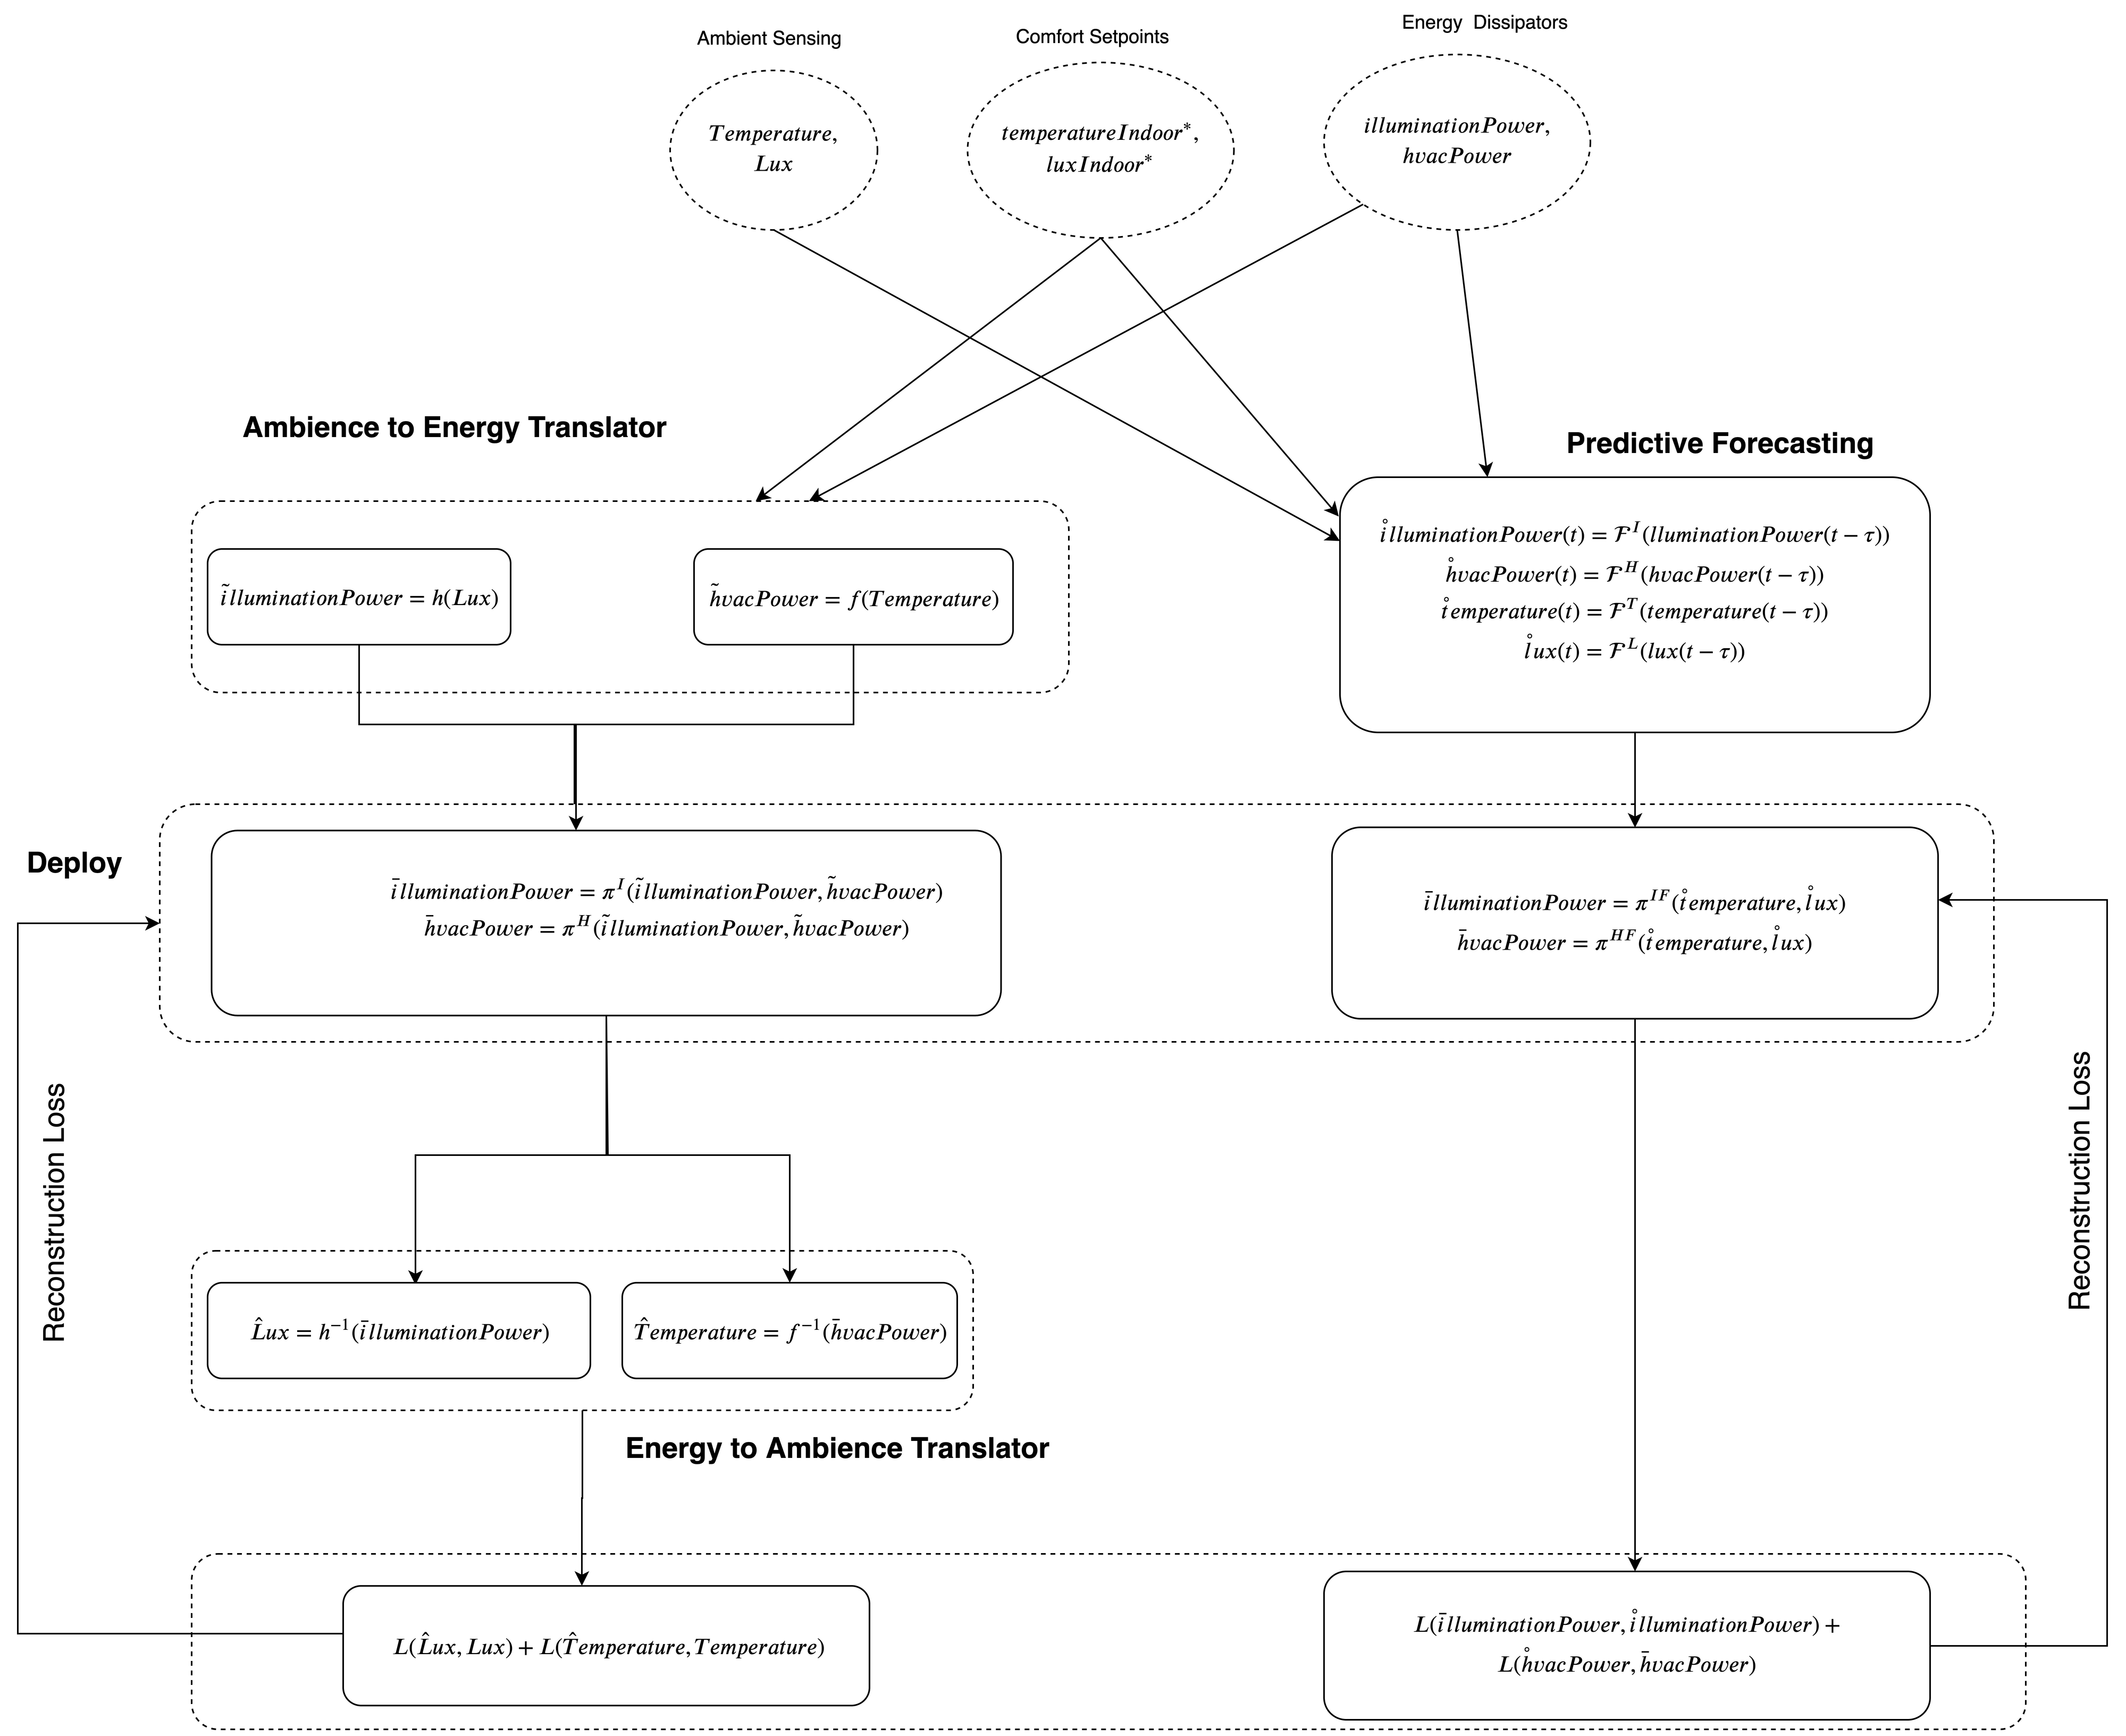
\includegraphics[width= 8cm]{img/LLequation.png}
    \caption{Overview of Functional Flow in NGIS}
    \label{fig:LLequation}
\end{figure}



=====================MAYBE Irelavant Below ==============
\subsection{}
\begin{figure}
    \centering
    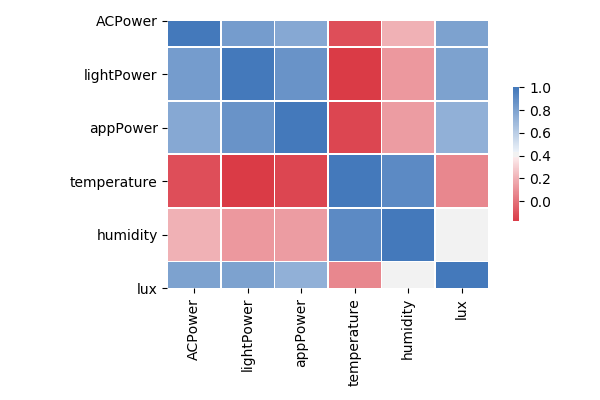
\includegraphics[width=\textwidth]{img/corr-z2-f2.png.png}
    \caption{Correlation Matrix between Sensors covering Zone 2}
    \label{fig:corr-z2-f2}
\end{figure}



\begin{figure}
\includegraphics[width=.4\textwidth]{x}{img/corr-z2-f2.png}\caption{Overview of Functional Flow in NGIS}
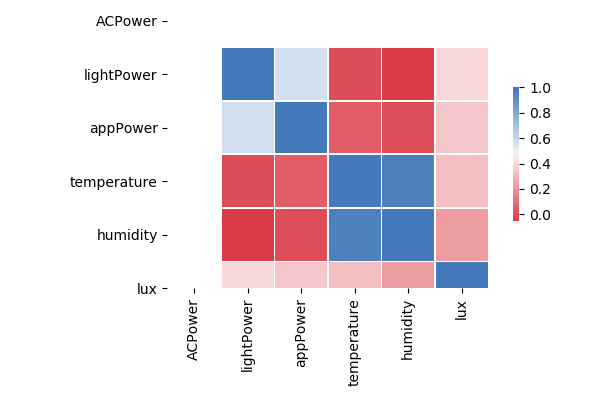
\includegraphics[width=.4\textwidth]{img/corr-z3-f2.png}\caption{Overview of Functional Flow in NGIS}
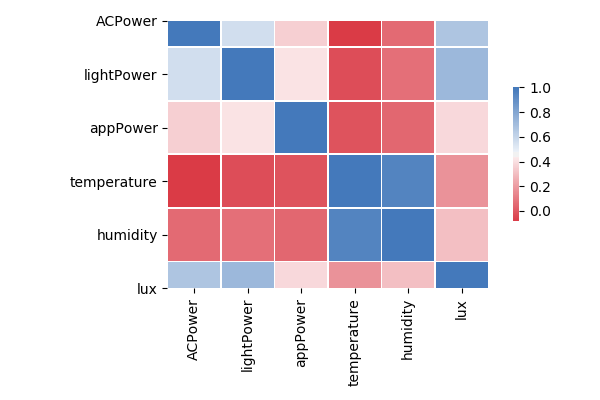
\includegraphics[width=.4\textwidth]{img/corr-z2-f7.png}
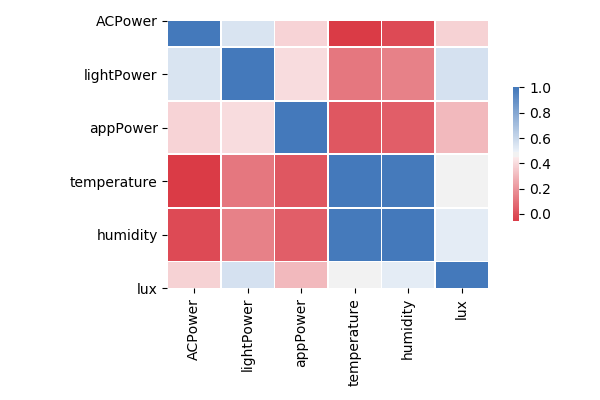
\includegraphics[width=.4\textwidth]{img/2018corr-z2-f7.png}
\caption{ 4 figures}
\end{figure}

 
 
 \begin{figure}%
    \centering
    \subfloat[Zone 2  1]{{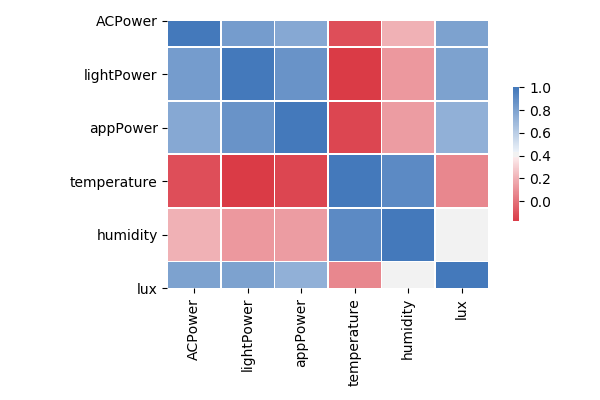
\includegraphics[width=0.47\textwidth]{img/corr-z2-f2.png} }}%
    \qquad
    \subfloat[\centering Zone 3 ]{{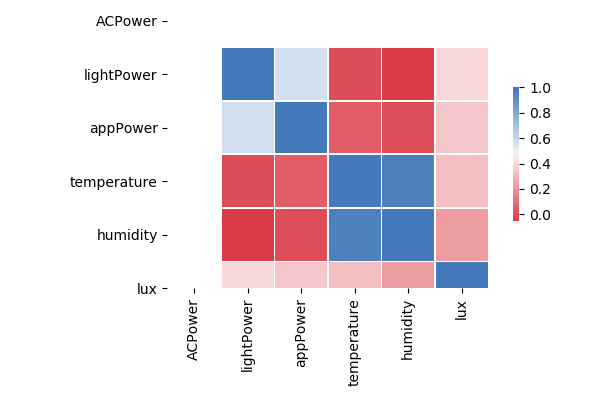
\includegraphics[width=0.47\textwidth]{img/corr-z3-f2.png} }}%
    \caption{Variation of sensor correlation matrix between two zones of Floor 2 in the building. }%
    \label{fig:diffzonesamefloorcomparision}%
\end{figure}


We choose a deep learning based forecasting model to skip the manual feature extraction for time series forecasting. 

If a zone is devoid of sensors, the set of deployed models are forecasting models and predictive policy learners $(\pi^{IF}, \pi^{HF})$ . 
In such a situation, there is no explicit feedback and hence no scope of improvement till data collection.
But in zones with sensors, whenever there is a prediction for time $t$, then comparison with the ground truth acts as a feedback. 
In a single task learning mode, this can improve the accuracy of the power allocation policy and additionally forecasting models (in joint mode).

The trade-off in replacing a sensor with it's forecasting counterpart is almost negligible if the approximating error over time stays within a permissible bound. 




\begin{figure}%
    \centering
    \subfloat[\centering 2018 data ]{{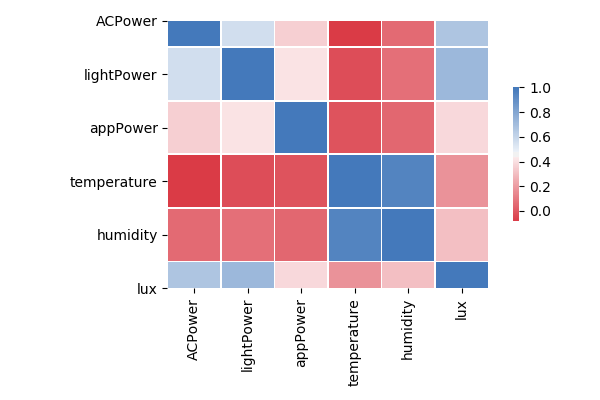
\includegraphics[width=0.47\textwidth]{img/corr-z2-f7.png} }}%
    \qquad
    \subfloat[\centering 2019 data 2]{{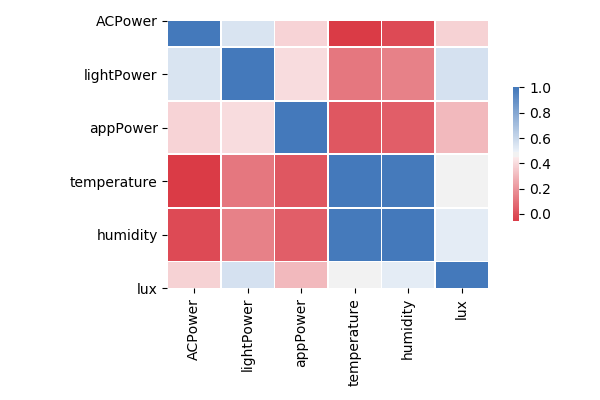
\includegraphics[width=0.47\textwidth]{img/2018corr-z2-f7.png} }}%
    \caption{Temporal deviation of correlation values between successive years of a zone.}%
    \label{fig:samezonetimecomparision}%
\end{figure}